\section{ErLam Toolkit}

\subsection{The Language}

\begin{slide}
    \begin{figure}
    \centering
        {\footnotesize
            %%
%% ErLam BNF Style Grammar.
%%
\begin{BVerbatim}[commandchars=\\\{\}]
<Expression> ::= <Variable> 
              |  <Integer>
              |  `\textbf{newchan}'
              |  `\textbf{(}' <Expression> `\textbf{)}'
              |  <Expression> <Expression>
              |  `\textbf{if}' <Expression> <Expression> <Expression>
              |  `\textbf{swap}' <Channel> <Expression>
              |  `\textbf{spawn}' <Expression>
              |  `\textbf{fun}' <Variable> `\textbf{.}' <Expression>
\end{BVerbatim}

        }
    \label{fig:grammer}
    \end{figure}

    \inote{
        \item Extremely simple on purpose (5 keywords).
        \item Issue now began to be how to build up test primitives
        \item Made a library which allowed for built ins.
    }
\end{slide}

\begin{slide}
    \begin{figure}
    \centering
    \begin{BVerbatim}
elib
    // ...
    ignore = (fun _.(fun y.y));
    omega = (fun x.(x x));
    // ...
    add = _erl[2]{ fun(X) when is_integer(X) ->
                        fun(Y) when is_integer(Y) ->
                            X+Y
                        end
                    end
                 };
    // ...
bile
    \end{BVerbatim}
    \end{figure}

    \inote{
        \item There's options for built-ins as well as macros.
        \item Built-ins are raw Erlang, gets wrapped up into AST, and still "reduces" the same (\ie~no multi-variable functions).
    }
\end{slide}

\begin{SaveVerbatim}{SimpleSwap}
(fun c.
     (ignore 
       (spawn (fun _.(swap c 42)))
       (swap c 0))
 newchan)
\end{SaveVerbatim}

\begin{slide}
    \framesubtitle{Example Application: Simple Swap}
    \begin{figure}
        \centering
        \BUseVerbatim{SimpleSwap}
    \end{figure}
    \begin{figure}
        \centering
        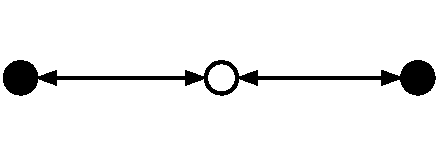
\includegraphics{SimpleSwap.pdf} 
    \end{figure}
    \inote{
        \item Here is a simple application which:
            \begin{itemize}
                \item Spawns a process to swap the number 42
                \item Calls swap to get the value from the other process.
            \end{itemize}
        \item Build up from here to simulate more complex behaviour.
        \item We can "do some work" before swaping, \etc
        \item This is how we built up or primitive test behaviours.
    }
\end{slide}

%\begin{SaveVerbatim}[commandchars=\\\{\}]{FibCode}
%// pfib.els -
%fun N.
%    (omega \textbf{fun} f,m.(
%        \textbf{if} (leq m 1) 
%           m
%           (merge \textbf{fun} _.(f f (sub m 1))
%                  \textbf{fun} _.(f f (sub m 2))
%                  add)) \textit{N})
%\end{SaveVerbatim}
%\begin{slide}
%\framesubtitle{Example Application: Parallel Fibonacci}
%    \begin{figure}
%    \centering
%    {\small
%        \BUseVerbatim{FibCode}
%    } 
%    \end{figure}
%    \begin{itemize}
%        \item[] {\tt \$ els pfib.els}\hspace{8.65mm}(Compile the script)
%        \item[] {\tt \$ ./pfib.ex -r 10}~~(Finds the 10th Fibonacci number)
%    \end{itemize}
%    
%    \inote{
%        \item R option is to run program applied to 10.
%        \item To add more to this presentation than just reading paper
%            I want to also give more detail as to system usage.
%        \item Explain this Common Usage Pattern.
%    }
%\end{slide}
%
%%%%%%%%%%%%%%%%%%%%%%%%%%%%%%%%%%%%%%%%%%%%%%%%%%%%%%%%%%%%%%%%%%%%%%%%%%%%%%
\subsection{Channel Implementations}

\begin{slide}
    \framesubtitle{Process Blocking Swap}
    \begin{figure}[t]
        \centering
        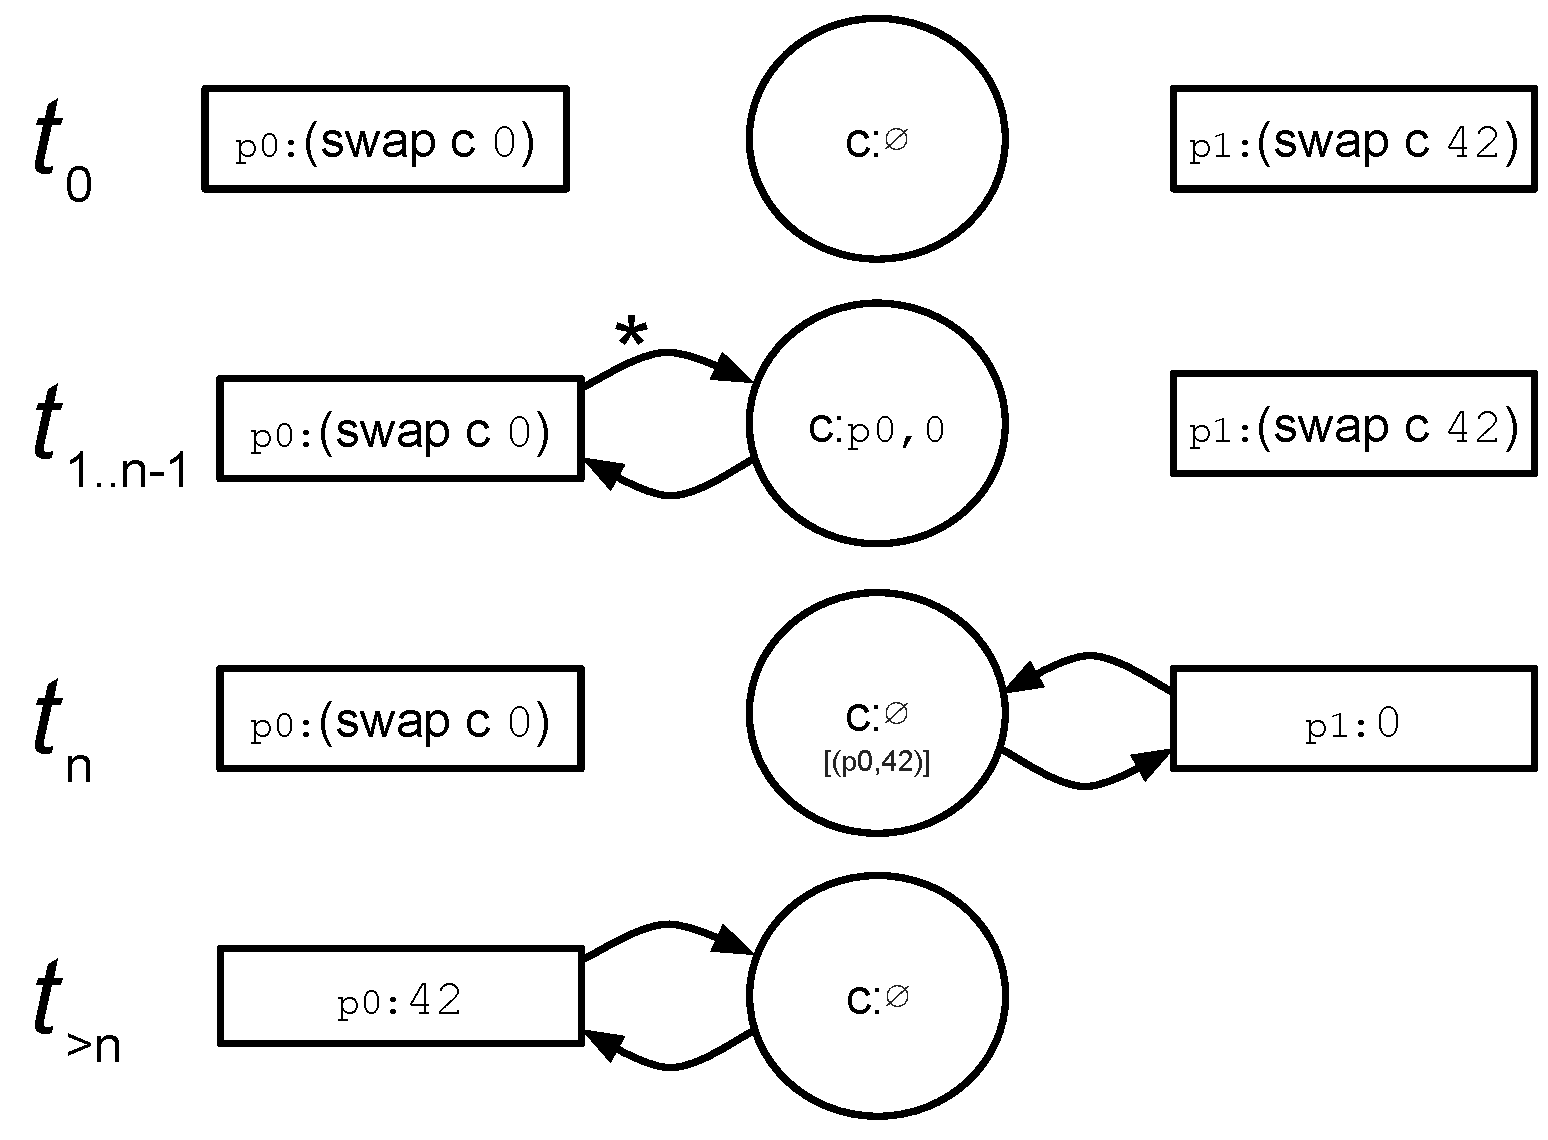
\includegraphics[width=0.8\textwidth]{BlockingSwap-verbose.pdf}
    \end{figure}
    
    \inote{
        \item Blocking: Maintains state of current and previous swap value until swap is completed.
        \item Mention expected effects on scheduler.
        \begin{itemize}
            \item Scheduler will keep hold of the process, needs to recheck if blocked.
            \item If all processes are communicating, large process queue of blocked processes. 
        \end{itemize}
    }
\end{slide}
\begin{slide}
    \framesubtitle{Process Absorption Swap}
    \begin{figure}[t]
        \centering
        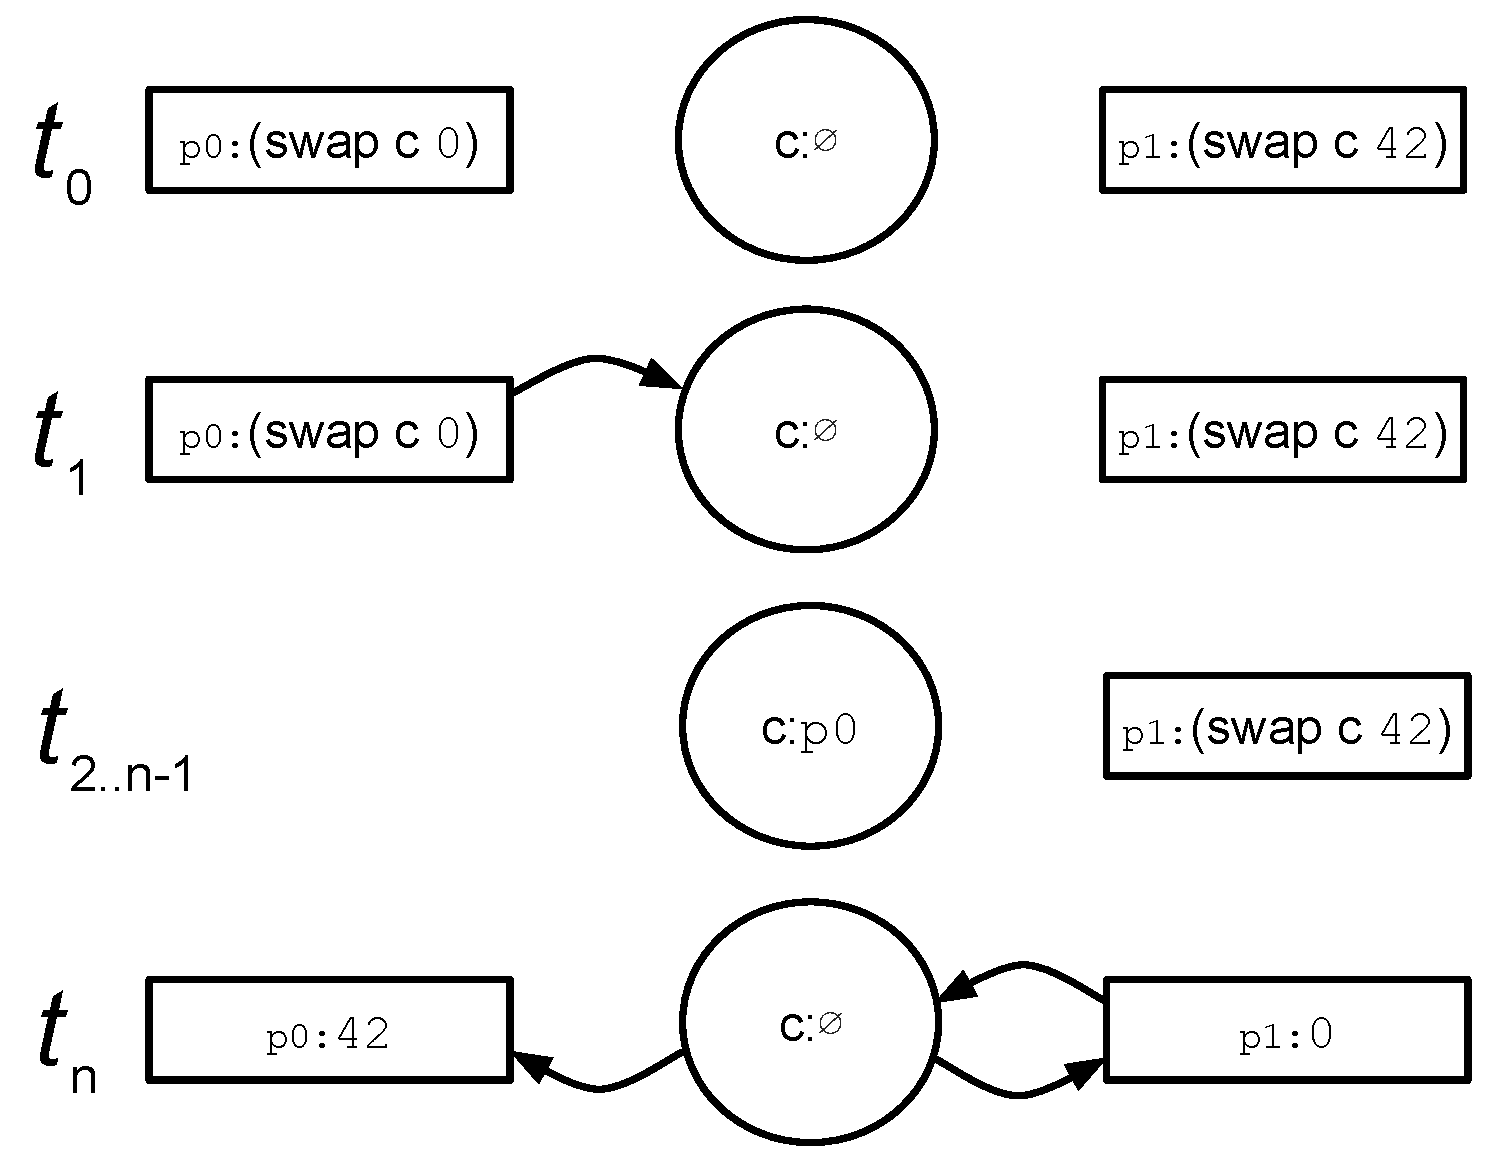
\includegraphics[width=0.8\textwidth]{AbsorbSwap-verbose.pdf}
    \end{figure}

    \inote{
        \item[1.] Whole process gets absorbed by channel, away from scheduler.
        \item[2.] When the second process completes the swap, the process gets
                  removed from channel.
            \begin{itemize}
                \item The p0 process can go back to its original scheduler, 
                \item OR to scheduler which unblocked it.
            \end{itemize}
        \item Effects on scheduler:
            \begin{itemize}
                \item Can loose or gain a extra process during communication.
            \end{itemize}
    }
\end{slide}

%%%%%%%%%%%%%%%%%%%%%%%%%%%%%%%%%%%%%%%%%%%%%%%%%%%%%%%%%%%%%%%%%%%%%%%%%%%%%%
\subsection{Simulation \& Visualization}

\begin{slide}
    System Behaviours:
            \begin{itemize}
                \item Degree of Parallelism
                \item Consistency of Cooperation
                \item Degree of Longevity/Interactivity
                \item Partial System Cooperativity
            \end{itemize}
    Logging \& Report Generation

    \inote{
        \item We first want to look at four types of system behaviour ranges:
            \begin{itemize}
            \item Parallelism: Gets back to Ring vs Cloud, Compare the two. 
            \item Consistency: Ring/Star=consistent, but if given a random choice.
            \item Longevity: Ratio of Communicating/Computing processes.
                \begin{itemize}
                    \item Longevity = Time spent reducing (low=communicator)
                    \item Interactivity, also takes into account user interaction.
                \end{itemize}
            \item Full vs Partial Cooperation: Multiple groups of Stars or Rings.
            \end{itemize}
        \item Definitely won't get to all behaviour tests that were in report, 
            but will focus on the key ones for each scheduler mechanic.
        \item Finally, quickly, go over the current report generation that 
            ErLam can perform.
    }
\end{slide}

\begin{slide}
    \framesubtitle{System Behaviours: Degree of Parallelism}
    \begin{figure}
        \centering
        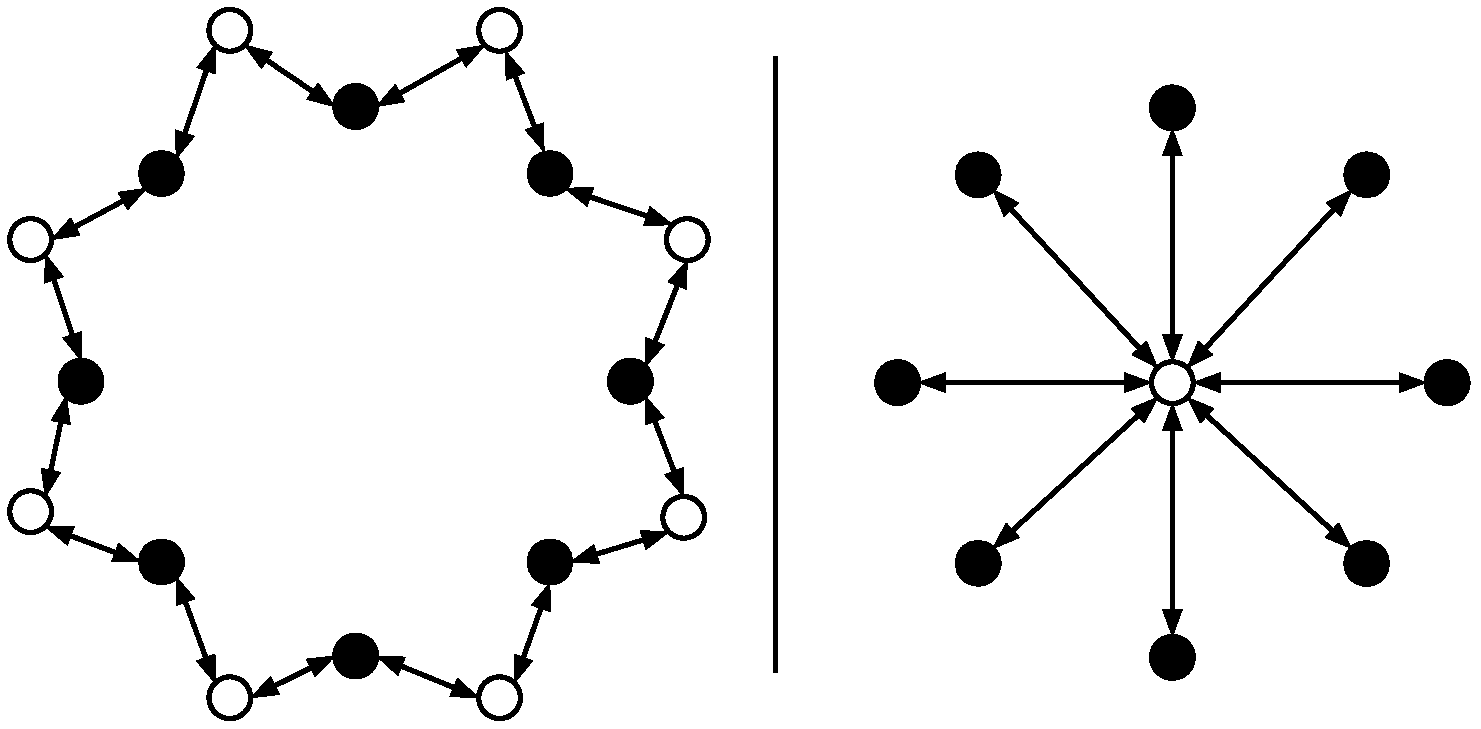
\includegraphics[scale=0.4]{RingVCluster.pdf}
        \caption{$PRing_N$, and $ClusterComm_{(N,1)}$ primitives to 
            test degree of parallelism.}
    \end{figure}

    \inote{
        \item Brings back the Ring and Star.
        \item We call the left, PRing, with the parameter N = number of processes. 
        \item We call the right, $ClusterComm$ with two parameters, $N$ like 
                $PRing$, $M=1$ in this cas
    }
\end{slide}

\begin{slide}
    \framesubtitle{System Behaviours: Consistency of Cooperation}
    \begin{figure}
        \centering
        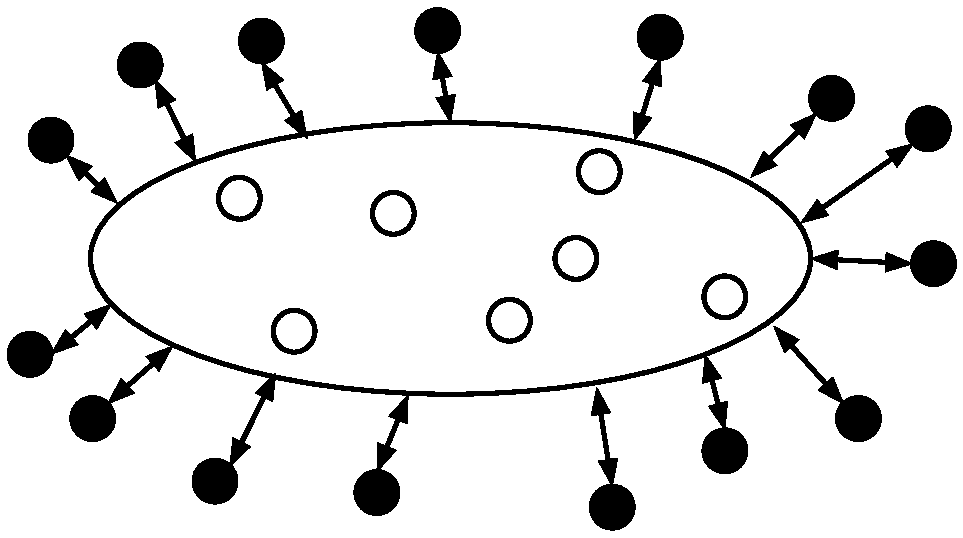
\includegraphics[scale=0.5]{ClusterComm.pdf}
        \caption{$ClusterComm_{(N,M)}$ to test effect of consistency on scheduler.}
    \end{figure}

    \inote{
        \item We can vary number of channels in relation to processes to 
            check the effects of inconsistency on Cooperative-Conscious schedulers.
        \item Worst case scenario for C-C schedulers. 
    }
\end{slide}

\begin{slide}
    \framesubtitle{System Behaviours: Degree of Interactivity}
    \begin{figure}
        \centering
        \only<1>{
            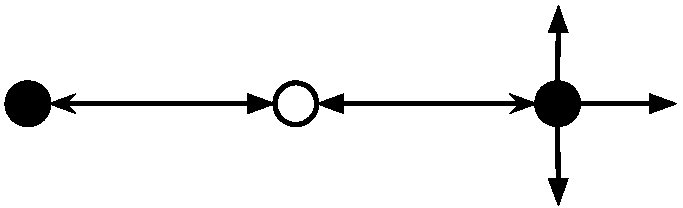
\includegraphics[scale=0.7]{UserInput.pdf}
            \caption{$UserInput_{(T,C)}$, simulates user interaction or a number 
                    ($C$) of external/timed ($T$) events.}
        }
        \only<2>{
            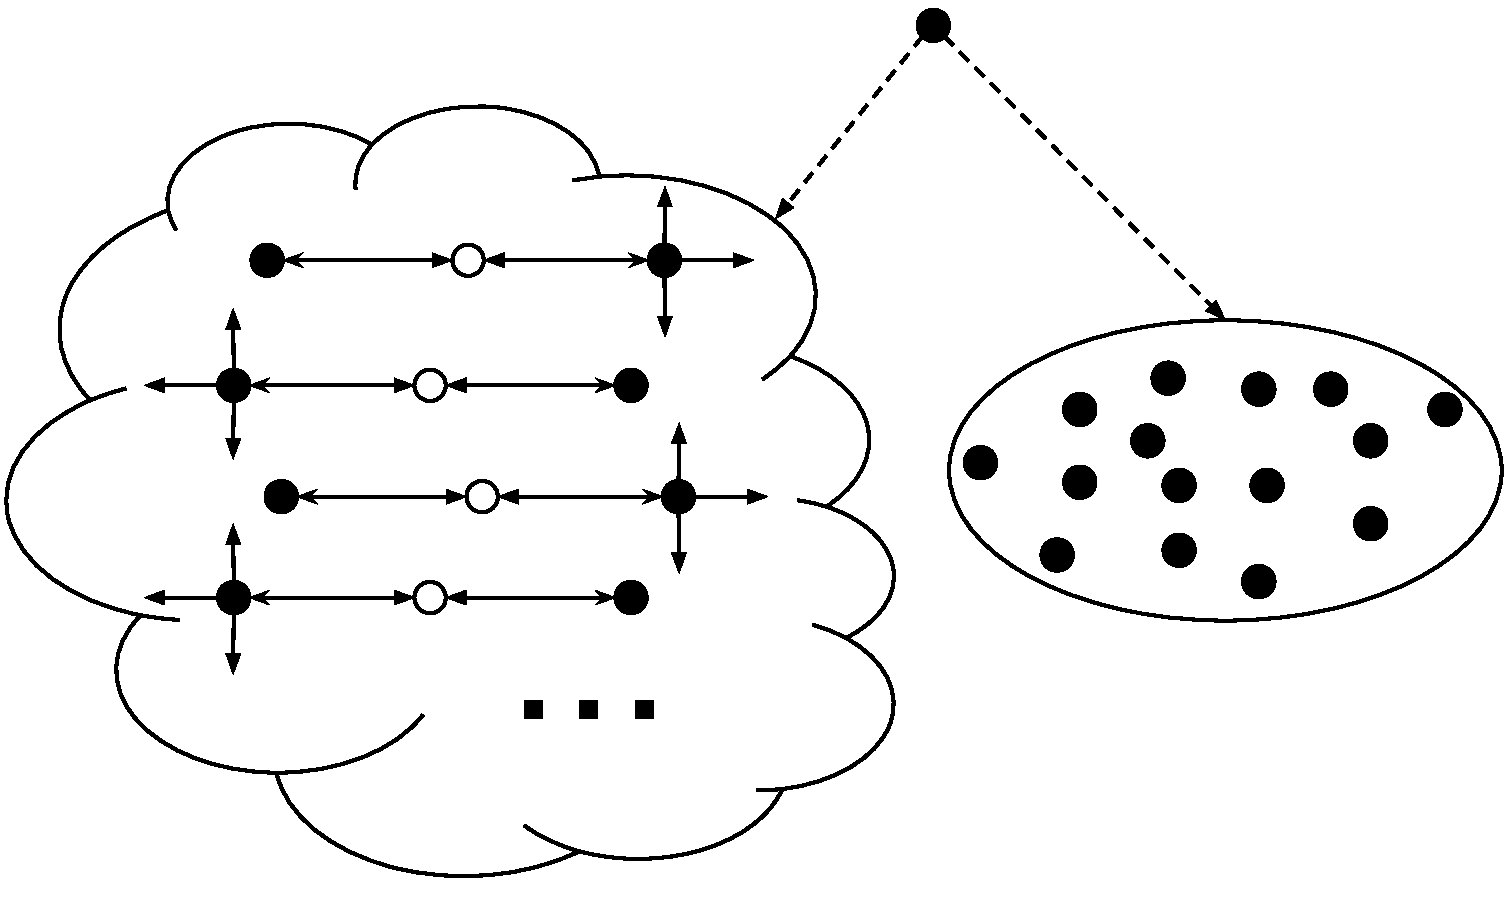
\includegraphics[scale=0.4]{Interactivity.pdf}
            \caption{$Interactivity_{(N,M)}$, composure of $ChugMachine_N$ (Cloud),
                    and $M$ instances of $UserInput_{(5,2)}$.}
        }
    \end{figure}
    
    \inote{
        \item To test longevity we can just vary the length of time the processes
            chug for all tests.
        \item To test interactivity though, we need a way to simulate user 
            interaction.
        \item $UserInput$ captures hanging for a single event. We can compose 
            these: $<NEXT>$
        \item With our cloud of processes (also called chugmachine) for 
            simulating a program with consistent working processes and 
            processes which are interactive.
    }
\end{slide}

\begin{slide}
    \framesubtitle{System Behaviours: Partial System Cooperativity}
    \begin{figure}
        \centering
        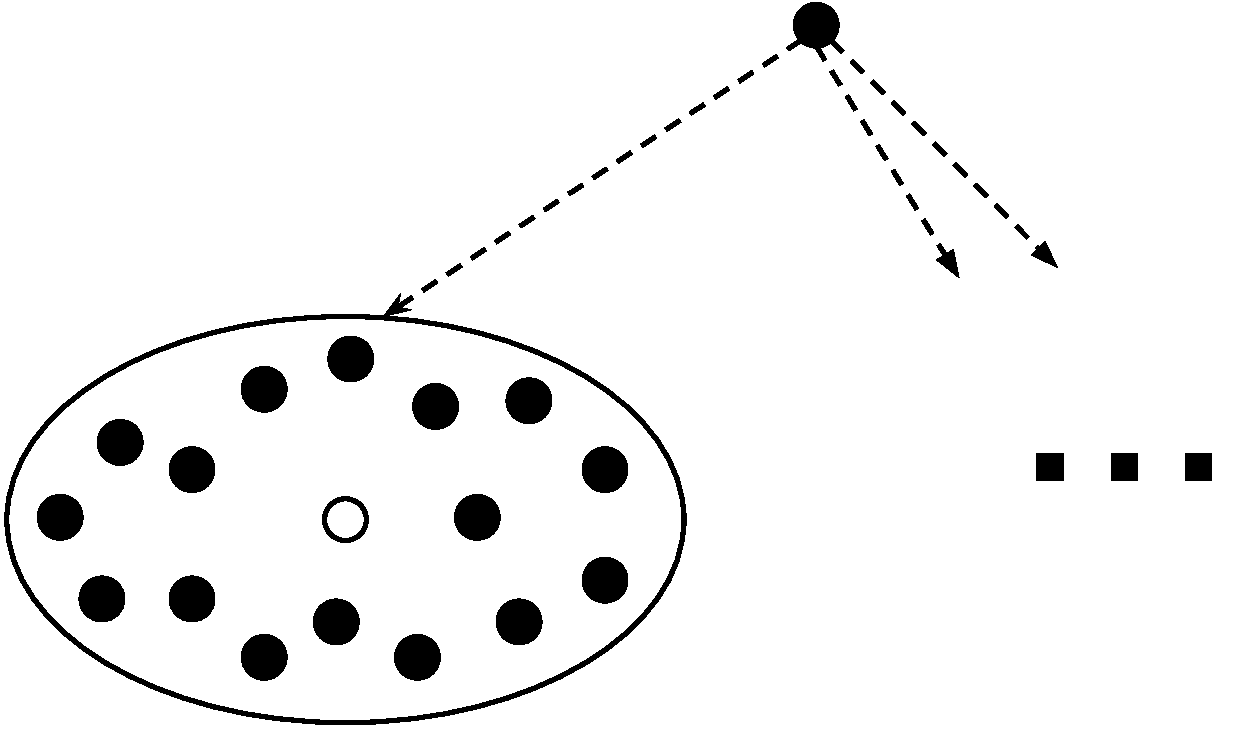
\includegraphics[scale=0.5]{PTree.pdf}
        \caption{$PTree_{(W,N)}$, a composure of $W$ $ClusterComm_{(N,1)}$ 
                instances running concurrently.}
    \end{figure}

    \inote{
        \item Previously (besides Interactivity), all systems were full system 
            cooperation.
        \item We can of course use Interactivity for our partial system 
            cooperativity tests, but we would instead like to see logical grouping.
        \item Hence the set of Work groups (or stars). 
    }
\end{slide}

\begin{slide}
    \framesubtitle{Logging \& Report Generation}

    Things we could log:
    \begin{itemize}
        \item Process Queue Size (per LPU)
        \item Quantity of Reductions/Yields/Preempts
        \item State of the Scheduler (waiting/running)
        \item Channel State (Blocked/Unblocked)
        \item \ldots
    \end{itemize}

    \inote{ % Notes are offset X+1 intentionally.
        \item Queue-Length: work-stealing mechanics and saturation ability.
        \item Tick-Action: Visualize the density of computation/communication.
        \item Sched-State: Useful for comparing stealing/process selection 
                  mechanics.
        \item Chan-State: Tracking interactivity, speed of unblock=attentive 
                  to cooperation. 
        \item Of course there are more, but we limited ourselves to the above 
                  for initial testing purposes. 
    }
\end{slide}

\begin{slide}
    \begin{figure}
        \begin{table}[t]
            \centering
            \begin{tabular}{@{}ccc}
                 \multicolumn{1}{c|}{\textbf{Queue Size}} &
                 \multicolumn{1}{c|}{\textbf{Reduc. Density}} &
                 \multicolumn{1}{c}{\textbf{Channel State}} \\ \cline{1-3}
            \multicolumn{1}{|c|}{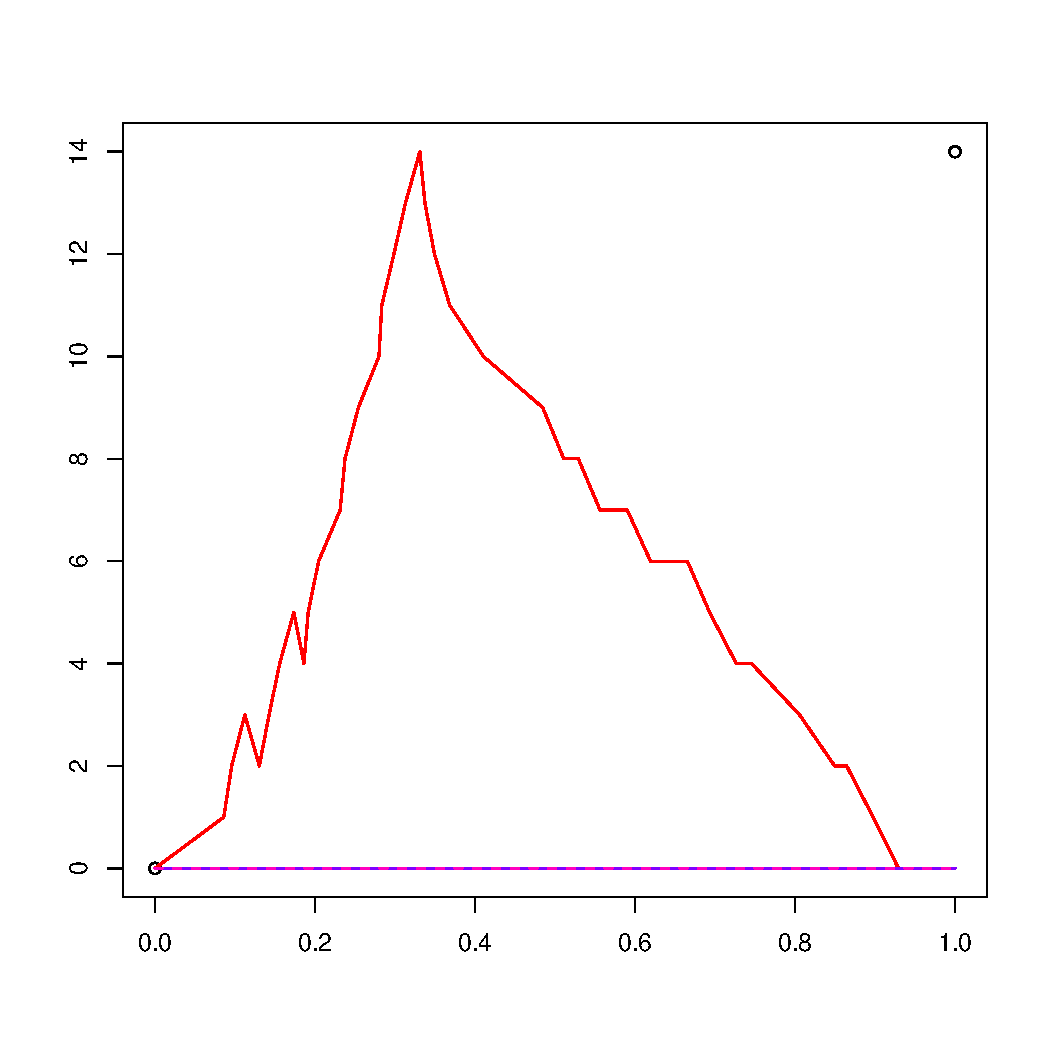
\includegraphics[scale=0.18]{tests/clustercomm/20/wssq/ca/pg_0003.pdf}} & 
            \multicolumn{1}{c|}{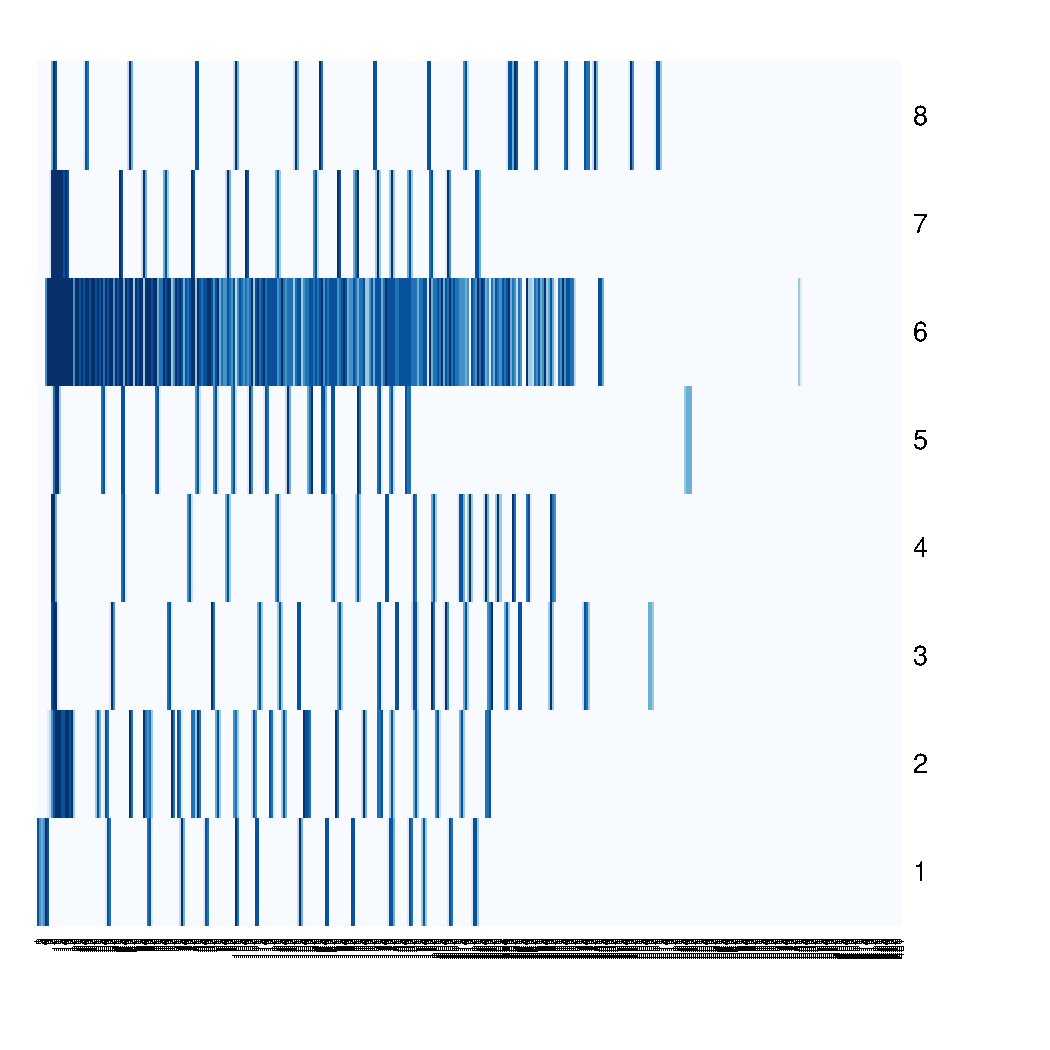
\includegraphics[scale=0.18]{tests/clustercomm/20/wssq/ca/pg_0004.pdf}} & 
            \multicolumn{1}{c|}{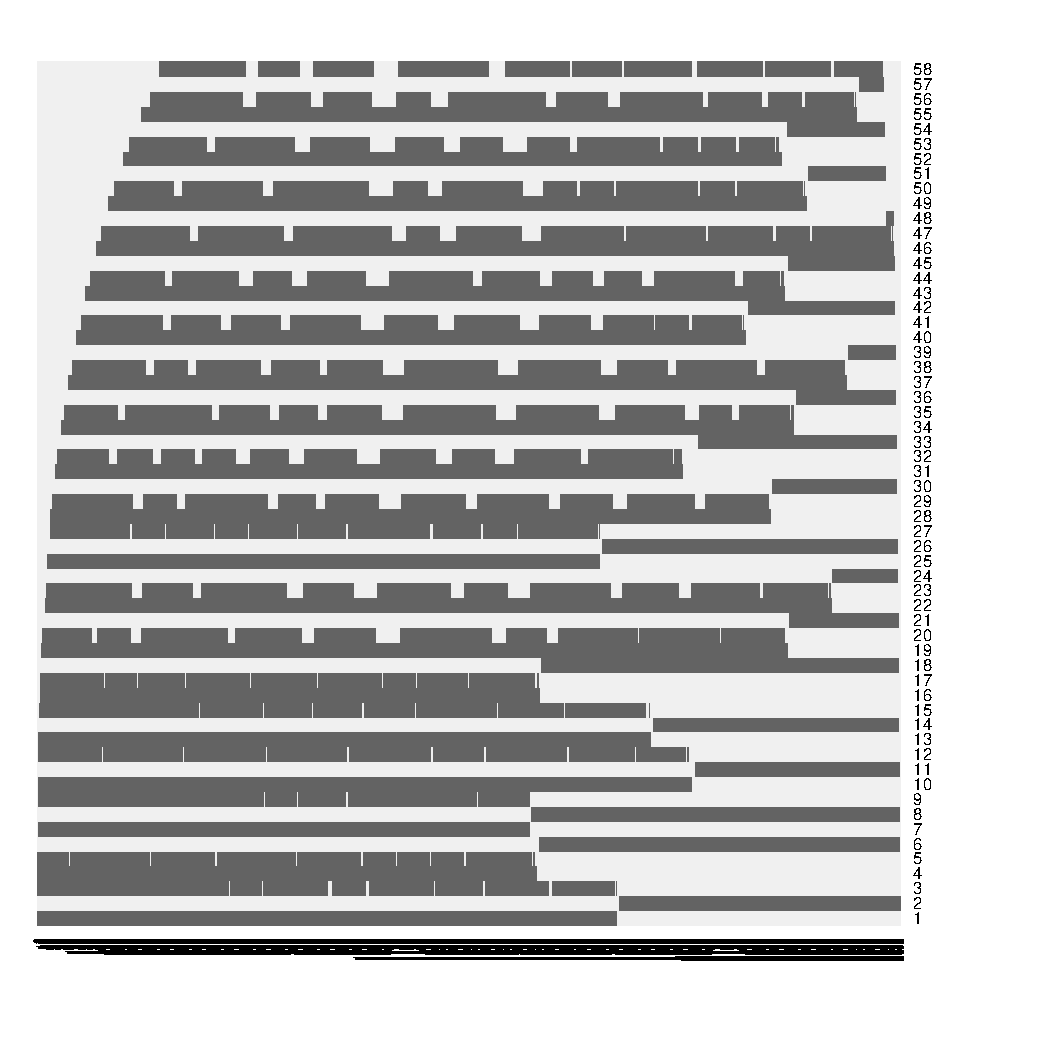
\includegraphics[scale=0.18]{tests/clustercomm/20/wssq/ca/pg_0001.pdf}} \\ 
            \cline{1-3}
            \end{tabular}
        \end{table}
    \end{figure}

    \inote{
        \item Three types of graphs:
        \begin{itemize}
            \item Queue Size: X-axis is time, Y-axis is size of queue
            \item Density charts: Darkness of the line represents fraction of ticks event happened in.
            \item Channel State: dark=blocked, light=unblocked. 
        \end{itemize} 
    }
\end{slide}

